\section{Quick Reference}
\subsection{Virtual Memory}
\begin{minted}{shell}
# vm virtual memory
# pm physical memory
# pg page
# vpn virtual page number
# ppn physical page number
# tlb table lookaside buffer
# wsa way set associative
# lvl level
# pte page table entry

# NOTE if not LRU is mentioned ignore tlb_entry_bits in tlb_size_bit

lvl_count
lvl_n_size_bytes
lvl_n_size_bits

# per level (unit is bits)
pte_n_size = (lvl_n_size_bytes / kiB) * align(ppn_size_bits + tlb_extra_bits)

# The sum of all lvl_n_size_bits adds up to vpn_size_bits
sum(pte_n_size for all n) = vpn_size_bits

wsa_count # ways
tlb_count # entries
tlb_sets       = tlb_count / wsa_count = 2^(tlb_sets_bits)
tlb_tag_bits   = vpn_size_bits - tlb_sets_bits
tlb_extra_bits = sum(...)
tlb_bits       = tlb_tag_bits + ppn_size_bits + tlb_extra_bits
tlb_set_ways   = wsa_count! = 2^(set_way_bits) # true LRU
tlb_entry_bits = ceil(set_way_bits) # true LRU
               = wsa_count - 1      # pseudo LRU
tlb_size_bit   = tlb_bits * wsa_count + tlb_entry_bits
tlb_storage    = tlb_sets * tlb_size_bit

lru_size_bits  = tlb_sets * tlb_entry_bits 

vm_size_bytes = vm_addr = 2^(vm_bits)
pm_size_bytes = pm_addr = 2^(pm_bits)
pg_size_bytes = pg_addr = 2^(pg_bits)

# offsets
vm_bits = vm_addr = log2(vm_size_bytes)
pm_bits = pm_addr = log2(pm_size_bytes)
pg_bits = pg_addr = log2(pg_size_bytes)
vm_tot_pg = vm_size_bytes / pg_size_bytes = 2^(vm_bits - pg_bits)
pm_tot_pg = pm_size_bytes / pg_size_bytes = 2^(pm_bits - pg_bits)

vpn_size_bits = log2(vm_tot_pg) = vm_bits - pg_bits
ppn_size_bits = log2(pm_tot_pg) = pm_bits - pg_bits
\end{minted}
\begin{minted}{markdown}
## Address Granularity Considerations

### Byte-Addressable Systems (common)
- Each address points to **one byte**
- Offset = log2(page size in **bytes**) = pg_bits

### Word-Addressable Systems
- Each address points to **one word** (e.g., 4 bytes or 8 bytes)
- Offset = log2(page size in **words**) = log2(page size in bytes) - log2(word size)

### Example
- **Byte-addressable** with 4 KB pages:
  - pg_bits = log2(4096) = 12 (offset = 12 bits)
- **Word-addressable** (4-byte words) with 4 KB pages:
  - pg_bits = log2(4096) - log2(4) = 12 - 2 = 10 (offset = 10 bits)
\end{minted}
\subsection{AMAT}
\begin{minted}{text}
AMAT= hit_time + miss_rate * miss_penalty
\end{minted}
Multiply through each node in a path and add all paths from root to
leaves.
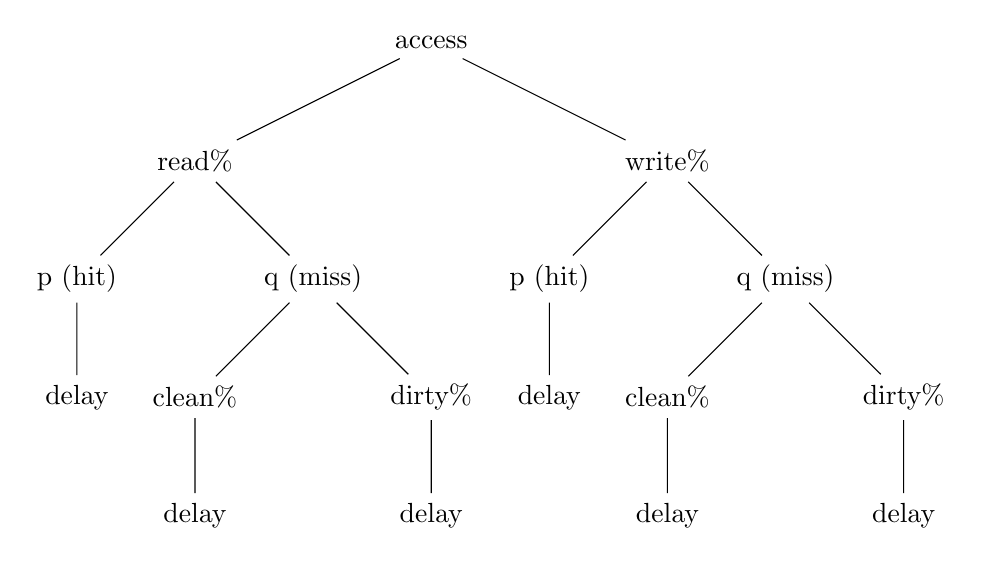
\begin{tikzpicture}[level distance=1.5cm,
    level 1/.style={sibling distance=6cm},
    level 2/.style={sibling distance=3cm}]
  \node {access}
  child {node {read\%}
      child {node {p (hit)} child {node {delay}}}
      child {node {q (miss)}
          child {node {clean\%} child {node {delay}}}
          child {node {dirty\%} child {node {delay}}}
        }
    }
  child {node {write\%}
      child {node {p (hit)} child {node {delay}}}
      child {node {q (miss)}
          child {node {clean\%} child {node {delay}}}
          child {node {dirty\%} child {node {delay}}}
        }
    };
\end{tikzpicture}

Example: cache hit \qty{30}{\nano\second}, cache miss
\qty{120}{\nano\second}, $75\%$ read rest are write, $70\%$ are
dirty rest are clean, and $95\%$ hit rate.

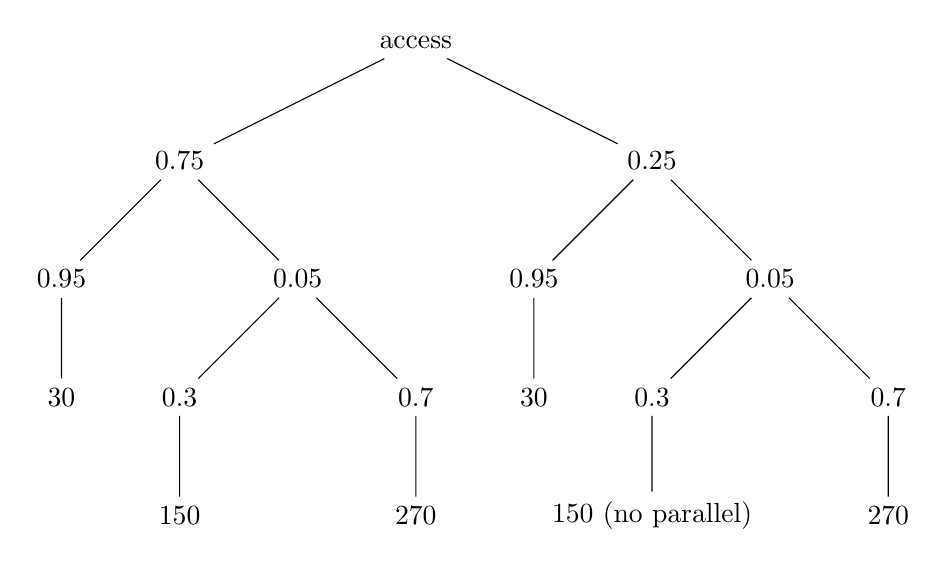
\begin{tikzpicture}[level distance=1.5cm,
  level 1/.style={sibling distance=6cm},
  level 2/.style={sibling distance=3cm}]
\node {access}
child {node {0.75}
    child {node {0.95} child {node {\qty{30}{\nano\second}}}}
    child {node {0.05}
        child {node {0.3} child {node {\qty{150}{\nano\second}}}}
        child {node {0.7} child {node {\qty{270}{\nano\second}}}}
      }
  }
child {node {0.25}
    child {node {0.95} child {node {\qty{30}{\nano\second}}}}
    child {node {0.05}
        child {node {0.3} child {node {\qty{150}{\nano\second} (no parallel)}}}
        child {node {0.7} child {node {\qty{270}{\nano\second}}}}
      }
  };
\end{tikzpicture}

\subsection{Endianness}
Integer value $0\times11~22~33~44$ at addess $0\times10$
\begin{center}
  \begin{tabular}{|l|r|r|r|r|}
    \hline
    address       & $0\times10$ & $0\times11$ & $0\times12$ & $0\times13$ \\
    \hline
    little endian & $0\times44$ & $0\times33$ & $0\times22$ & $0\times11$ \\
    \hline
    big endian    & $0\times11$ & $0\times22$ & $0\times33$ & $0\times44$ \\
    \hline
  \end{tabular}
\end{center}
\subsection{CPU Timing}
where T is CPU time, IC are total instructions, CPI is cycles per
instruction, and CT is cycle time:
$$\mathrm{T}=\mathrm{IC}\cdot\mathrm{CPI}\cdot\mathrm{CT}$$
